%\documentclass{article}
%\documentclass[dvips,11pt,a4paper]{article}
\documentclass[a4paper]{article}

\usepackage{xspace}
\usepackage{graphicx}
\usepackage{wrapfig}
%\usepackage{doublespace}
\usepackage{setspace}
%\usepackage{boxedminipage}

% \newcommand{\QOSR}{QoS routing}
\newcommand{\ie}{i.e.,\xspace}
\newcommand{\eg}{e.g.,\xspace}
\newcommand{\cf}{c.f.,\xspace}

\newenvironment{problem}[1]%
{\noindent{}\textsc{Problem #1}: }{\vspace{12pt}}


\setlength{\hoffset}{0pt}
\setlength{\voffset}{0pt}
\setlength{\oddsidemargin}{0pt}
\setlength{\textwidth}{16cm}
\setlength{\topmargin}{-37pt}
\setlength{\textheight}{670pt}
\setlength{\footskip}{60pt}



\begin{document}
\title{Introduction to Routing in general,\\Shortest--path routing \& Quality--of--Service routing}
\author{Lars Staalhagen \\ Networks Incompetence Area \\ Research Center
  COM \\ ls@com.dtu.dk }
\date{\small{}Version 0.1 --- \today}
\maketitle

\section{Introduction}
The purpose of this lecture note is to introduce two concepts in
routing: Shortest--path routing and Quality--of--Service routing. It
is intended to be used in course 34355 Routing in Data Networks.

The lecture note is structured as follows: In section XXXX the
concept of shortest--path routing is described, along with two
common algorithms for finding the shortest--paths in a network. In
section XXXX the Quality--of--Service routing (QoS--routing) is
described, starting with a general definition of QoS and QoS
routing. In the following two sections, some problems of
QoS--routing in relation to multicasting and ad--hoc networks are
described.

% \section{Routing in general}

\subsection{Definitions}
\begin{itemize}
%
\item\emph{Routing} -- Determining a path from a source to a destination.
%
\item\emph{Switching} -- The process in a network node of receiving a piece of information on an input interface and sending the information out on an output interface
%
\item\emph{Router} -- A node/device in a network that performs routing and switching. Usually associated with layer 3 (the network layer) in the OSI reference model.
%
\item\emph{Routing protocol} -- A protocol for exchanging information between routers, to permit these to perform routing
%
\item\emph{Routing table} -- A table maintained in a router that can lists the next--hop as a function of the destination identity.
%
\item\emph{Source routing} -- Routing where packets contain the full path from the source to the destination in their header.
%
\item\emph{Hop--by--hop routing} -- Routing, where the packets only contain the identity of the destination node, and where the routers then determine the next--hop from the routing table.
%
\item\emph{Static and dynamic routing} -- In static routing, the paths through the network are determined at network initialization. These paths are not changed unless required, e.g. by a change of the network topology. In dynamic routing, the paths are continually updated.
%
\item\emph{Distributed vs. Centralized routing} -- In centralized routing, there is one node that is responsible for all path calculations. In distributed routing, every router makes a decision.
%
\item\emph{Flat vs. Hierarchical routing} -- In flat routing, the path calculations take every part of the network into account, while in hierarchical routing, the network is divided into different domains. In the latter case, this means that two kinds of routing must be handled: intra--domain routing and inter--domain routing.
%
\end{itemize}

\subsection{Some special routing principles}

\subsubsection{Flooding}

\subsubsection{Deflection routing}



\section{\label{sec:shortestpath}Shortest path routing}
The aim of shortest--path routing\footnote{In some textbooks, the term
  \emph{least--cost} routing is used instead.} is to find an optimal
path in a network from a source node to a destination node.

The algorithms that are used to determine such an optimal path assume a
graph--representation of the network, i.e., $G = (N,V)$, where $N$
are the nodes in the graph and $V$ are the edges\footnote{Other
names are \emph{arcs} or \emph{lines}}. The nodes in the graph corresponds to routers in the real network, while the edges in the graph correspond to links between routers. 

Since communication links can be either unidirectional (communication is only possible in one direction) or bidirectional (communication is possible in both directions), this must also be represented in the graph. In addition, a bidirectional link may be asymmetric in some sense, \ie the communication in the two directions may have different characteristics, \eg different delays.

Therefore, the graph that is used to represent a network will be a \emph{weighted directed} graph. Every edge is associated with a metric (a number), which represent some characteristic of the link in the real
network.

If a physical link is bidirectional, and has the same metric in both directions, it is common to draw the edge as "directionless", \ie without an arrowhead, but it must be kept in mind, that this edge actually represents two directional edges.

The metrics that are associated with the edges in the graph can be thought of as the \emph{length} of that edge. Therefore, a path from one node to another in the graph has a total length of the sum of the length of the edges that are part of the path. In this sense, the metrics are \emph{additive}.

The purpose of shortest--path routing is then to find paths in the graph that minimizes the path--lengths. The simplest problem would be to find the shortest--path from a given source--node to a given destination--node, but the common algorithms today determine the shortest--paths from a given source node to \emph{all} other nodes in the graph. A number of algorithms exists that can be used to determine the shortest paths, but in connection with communication networks, the most common are the \emph{Bellman--Ford} algorithm and the
\emph{Dijkstra} algorithm. The former is used in connection with the
RIP protocol, while the latter is used with the OSPF protocol. 

As described earlier, the metrics associated with the edges in the graph correspond with some characteristic of the physical link in the network. Examples of these metrics include:
\begin{itemize}
\item Delay -- the metric is (directly) proportional with the delay on
  the link, so that the shortest--path from the source to the
  destination is the path that minimizes the end--to--end delay. The
  link--delay may include any buffering delay at the sending node.
\item Economical cost -- the metric is (directly) proportional with
  the expenditure of transmitting information on the link. The
  shortest--path is then the path that minimizes the expenditure for
  the network operator.
\item Error rate -- the metric is a function of the link's error
  rate\footnote{Note that the metric and the link's error rate are not
    directly proportional in this case.}, so that a link with a high
  error--rate is depicted in the graph as an edge with a high
  cost. Finding the path in the graph that minimizes the sum of the
  edge metrics would then tend to favour links with lower error rates,
  since they would have a smaller metric.
\end{itemize}
In general, the link metrics may also be a function of (some of) the
parameters of a link, i.e.
\[
\textrm{Metric} = f(\textrm{delay}, \textrm{economical cost}, \ldots)
\]

%Figure~\ref{fig:Graphs} illustrates an undirected and a directed graph.
%\begin{figure}[ht]
%\centering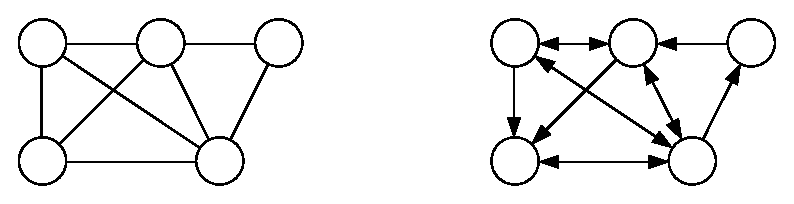
\includegraphics{Graphs}
%\caption{\label{fig:Graphs}Undirected and directed graph.}
%\end{figure}

In mathematical terms, the link--metrics are here denoted by $C_{ij}$
for the metric on the link \emph{from} node $i$ \emph{to} node $j$. In
general, $C_{ij}\ne{}C_{ji}$, i.e. for a bidirectional link, the
metrics are different in the two directions. This might be the case if
the metrics are a function of the link delays. By definition,
$C_{ii}=0$, since (informally) the distance from node $i$ to node $i$ is of course 0. Furthermore, two different nodes, $i$ and $j$, might not have a direct edge between them, so it is impossible to send a packet directly from node $i$ to node $j$.
This situation is represented in the metrics as $C_{ij}=\infty$.

The results of the shortest--path calculations are stored in the
source--node's routing table. If the network uses
\emph{source--routing}, the entire paths are stored since they
must be included in the packets. If the network uses
\emph{hop--by--hop} routing, the source node will only need to
store the identity of the next--hop node for all destinations.

\subsection{Bellman--Ford's algorithm}
The Bellman--Ford algorithm can be described as follows:

\setlength{\fboxsep}{9pt}
\begin{center}\noindent\fbox{\begin{minipage}[h]{0.9\textwidth}
\paragraph{Definitions:}
$s$ = Source node. $D^{h}_{j}$ = The cost of shortest path from $s$ to node $j$ under the condition, that the path contains at most $h$ links.
\vspace{9pt}
\paragraph{Initialization:}
$\forall h: D^{h}_s = 0$ and $\forall j\neq{}s:D^{0}_j =  \infty$
\vspace{9pt}
\paragraph{Iteration:}
$\forall j : D^{h+1}_{j} = \min_{k}\left(D^{h}_k + C_{kj}\right).$ Keep repeating the iteration until $\forall j: D^{h+1}_j = D^{h}_j$
\end{minipage}}
\end{center}

Consider the graph in figure~\ref{fig:Graphs2}.
\begin{figure}[ht]
\centering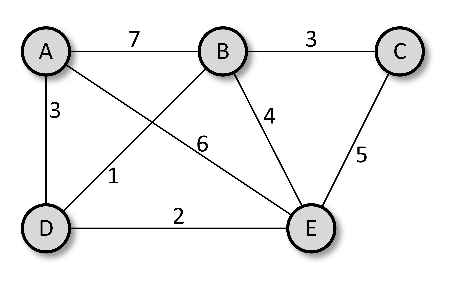
\includegraphics{Graphs2.eps}\caption{\label{fig:Graphs2}Example
network.}
\end{figure}

\noindent{}If we want to calculate the shortest paths from node A
to all other node in this network we get the following table:

\begin{table}[ht]
\centering
\begin{tabular}{|c|c|c|c|c|c|c|c|c|}\hline
%
 & \multicolumn{2}{|c|}{Node B} & \multicolumn{2}{|c|}{Node C} & \multicolumn{2}{|c|}{Node D} & \multicolumn{2}{|c|}{Node E} \\ \hline
%
$h$ & $D^{h}_B$ & Path & $D^{h}_C$ & Path & $D^{h}_D$ & Path &
$D^{h}_E$ & Path \\ \hline
%
0 (Init) & $\infty$ & --- & $\infty$ & --- & $\infty$ & --- &
$\infty$ & --- \\ \hline
%
1 & 7 & A--B & $\infty$ & --- & 3 & A--D & 6 & A--E \\
\hline
%
2 & 4 & A--D--B & 10 & A--B--C & 3 & A--D & 5 & A--D--E \\
\hline
%
3 & 4 & A--D--B & 7 & A--D--B--C & 3 & A--D & 5 & A--D--E \\
\hline
%
4 & 4 & A--D--B & 7 & A--D--B--C & 3 & A--D & 5 & A--D--E \\
\hline
\end{tabular}
\caption{Bellman-Ford calculation of shortest paths}
\end{table}

\noindent{}Since $D^{4}_{j} = D^{3}_{j}$ for all $j$, the
algorithm has converged. The routing table for node A will then
be:
\begin{table}[!ht]
\centering
%\begin{minipage}[c]{\textwidth}
%\centering \vspace{9pt}
\begin{tabular}{|c|c|c|}\hline
%
Destination & Path (source--routing) & Next--hop (hop--by--hop
routing) \\ \hline
%
B & A--D--B & D \\ \hline
%
C & A--D--B--C & D \\ \hline
%
D & A--D & D \\ \hline
%
E & A--D--E & D \\ \hline
\end{tabular}
\caption{Contents of routing table for source node.}
\end{table}
%\vspace{9pt}
%\end{minipage}

At this point, the shortest--paths from the source node to all
other nodes in the network have been found, but in general, we
need the shortest--paths between any pair of nodes in the network.
For this, it is necessary to execute the Bellman--Ford algorithm
$N$ times, where using (in turn) every node in the network as the
source node.

\subsection{Distributed Bellman--Ford}
\noindent{}The Bellman--Ford algorithm can also be implemented in
a distributed fashion. To implement this, a node must from time to
time transmit information from its entire routing table to all its
neighbor nodes. It can be shown that as long as all nodes from
time to time transmit this information, the optimal
shortest--paths will be determined eventually.

The idea behind the distributed Bellman--Ford is that, whenever a
node receives information from a neighbor node, it will determine
whether the information will lead to a better (smaller cost) path
than previously known. As an example, consider
figure~\ref{fig:Dist_BF_Ex}: Suppose that node A receives the
following information from node B: "I can reach node Z with a cost
of $\alpha$" and from C: "I can reach node Z with a cost of
$\beta$". Node A would then determine, which of these possible
ways of reaching node Z would be better by determining the minimum
of $C_{AB} + \alpha$ and $C_{AC} + \beta$. If $C_{AB} + \alpha <
C_{AC} + \beta$ then the (currently) best path from A to Z is via
node B; otherwise it is via node C.

\begin{figure}[!ht]
%\begin{wrapfigure}{r}{4in} \centering
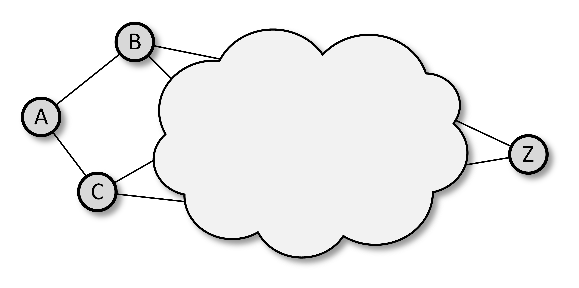
\includegraphics{Dist_BF_Ex.eps}
\caption{\label{fig:Dist_BF_Ex}Example network for the distributed
Bellman--Ford.}
\end{figure}
%\end{wrapfigure}


\subsection{Dijktra's algorithm}
Dijkstra's algorithm can be described as follows:

\begin{center}\noindent\fbox{\begin{minipage}[h]{0.9\textwidth}
\paragraph{Definitions:}
$s$ = source node. $D_j$ = (estimate) of the cost of the shortest
path from $s$ to (destination) node $j$. $N$ = set of all nodes in
the network. $M$ = set of nodes. \vspace{9pt}
\paragraph{Step 1:}
Initialize the set $M$ with just the source node, $M=\{s\}$
\vspace{9pt}
\paragraph{Step 2:}
Find the node with the smallest $D_j$ that is not yet included in
the set $M$ and add this node to $M$: $D_k = \min_{j \not\in M}
D_j$. $M \gets M \cup \{k\}$ \vspace{9pt}
\paragraph{Step 3:}
For all nodes not (yet) included in $M$, check if a path through
the just--added node (node $k$) would be better than the current
path. $D_j = min(D_j, D_k + C_{kj})$ \vspace{9pt}
\paragraph{Step 4:}
If $N\neq{}M$ continue from step 2; otherwise the algorithm has terminated.
\end{minipage}}
\end{center}

\noindent{}If we use Dijkstra's algorithm on the network in
figure~\ref{fig:Graphs2}, we get table~\ref{tbl:dijkstra}. The
routing table of node A will of course be the same as in the
Bellman--Ford example.

\begin{table}[ht]
\centering\begin{tabular}{|c|c|c|c|c|c|c|c|c|}\hline
 & \multicolumn{2}{|c|}{Node B} & \multicolumn{2}{|c|}{Node C} & \multicolumn{2}{|c|}{Node D} & \multicolumn{2}{|c|}{Node E}
 \\ \hline
$M$ & $D_B$ & Path & $D_C$ & Path & $D_D$ & Path & $D_E$ & Path \\
\hline
%
$\{A\}$ & 7 & A--B & $\infty$ & --- & 3 & A--D & 6 & A--E \\
\hline
%
$\{A, D\}$ & 4 & A--D--B & $\infty$ & --- & 3 & A--D & 5 & A--D--E
\\ \hline
%
$\{A, B, D\}$ & 4 & A--D--B & 7 & A--D--B--C & 3 & A--D & 5 &
A--D--E \\ \hline
%
$\{A, B, D, E\}$ & 4 & A--D--B & 7 & A--D--B--C & 3 & A--D & 5 &
A--D--E \\ \hline
%
$\{A, B, C, D, E\}$ & 4 & A--D--B & 7 & A--D--B--C & 3 & A--D & 5
& A--D--E \\ \hline
%
\end{tabular}
\caption{\label{tbl:dijkstra}Dijkstra calculation of shortest
paths}
\end{table}

\section{\label{sec:QoSR}Quality--of--Service Routing}

\subsection{Quality--of--Service concept}
The concept of \emph{Quality--of--Service} (QoS) has received a
lot of attention in recent years with increased interest in
distributed multimedia applications. These applications require
that the flow of information between the application participants
receives some kind of special treatment inside the network.
Examples include:
\begin{itemize}
%
\item \emph{Interactive applications} -- In this case, the total
delay experienced inside the network must be below some upper
bound.
%
\item \emph{Streaming applications} -- In this case, the flow must
receive a minimum throughput, and also required an upper bound on
the delay jitter, to minimize the buffer requirements in the
end--nodes.
%
\end{itemize}

In this lecture note, we will use the following definitions, from~\cite{ref:rfc2386}:
\begin{quote}
\textbf{Quality--of--Service (QoS):} A set of service requirements
to be met by the network while transporting a flow.\\
\textbf{QoS-based routing:} A routing mechanism under which paths
for flows are determined based on some knowledge of resource
availability in the network as well as the QoS requirement of
flows.
\end{quote}

Note that the previous definitions are related specifically to the
Internet, but we can here generalize to any kind of network.

The QoS--requirements of the applications can be translated into
two types of constraints:\begin{itemize}
%
\item \emph{Path--constraints} -- which are constraints on an
entire path through the network, but does not specify any
constraints on the individual links that are part of the path. An
example of a path--constraint is a requirement by the application
that the end--to--end delay must be smaller than some value, $D$.
In this example, the individual link--delays are not important,
just as long as the sum of all the link--delays are below $D$
%
\item \emph{Link--constraints} --  which are constraints that
every link in a path must satisfy. An example is the free
capacity of a link. If an application wishes to transfer a flow of
information with a minimum bitrate of $R$ bps, every link in the
path from the source node to the destination node must have an
free capacity of at least $R$ bps.
%
\end{itemize}

Given a number of constraints, the purpose of a QoS routing
algorithm is then to find an optimal path through the network. In
general, there might be a number of paths that all satisfies all
constraints -- these are called \emph{feasible paths} -- so the
QoS routing algorithm must select one of these based on some other
criteria.

\subsection{More on metrics}
The shortest--paths algorithms discussed in the previous section
were based on a graph representation of the real network. This
graph description is also relevant in connection with QoS--routing.

In the previous case, an edge in the graph was associated with
\emph{one} (additive) metric. In QoS--routing in general, an edge is now associated with \emph{multiple} metrics. As before, a metric may be additive, but in addition, in QoS--routing, we may also encounter metrics that are
\emph{non--additive}. A typical example is the free capacity
of a link. For instance, consider figure~\ref{fig:ResidualCapacityExample}. Suppose that the free capacity on the link A--B is 10 Mbps, while the free capacity on the link B--C is 6 Mbps. The throughput from A to C is definitely not 16 Mbps, but only 6 Mbps, i.e. the minimum of the residual capacities of the links in the path.
\begin{figure}[ht]
\centering
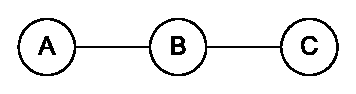
\includegraphics{ResidualCapacityExample.eps}
\caption{\label{fig:ResidualCapacityExample}Path with different
available bandwidths.}
\end{figure}

Another example of a non--additive metric is \emph{policies}, \ie
the network operator can impose policies on the links in the
network, so that for a given flow, only a subset of all the links
may be used.

The first step in QoS--routing is often referred to as \emph{topology filtering}. Here, edges with non--additive metrics that do not satisfy constraints are simply removed from the graph. In addition, any nodes that have become isolated are also removed. As an example: suppose that an information flow requires a minimum throughput of $D$ bps. In that case, any edge, where the free capacity is less than $D$ bps can simply be removed from the graph, since they could be part of any feasible path.

When constraints related to non--additive metrics have been
satisfied, the goal of a QoS routing algorithm is to find paths
that satisfies the constraints related to the additive metrics. At
this point, if there is only one constraint left, the problem can
be solved with any of the previously discussed shortest--paths
algorithms.

However, if there are multiple (additive) constraints left, finding the
optimal path is unfortunately NP-complete.




\section{\label{sec:M-QoSR}QoS Multicast Routing}
\framebox{\begin{minipage}{0.9\textwidth}\emph{General discussion
about the issues concerning QoS--routing in multicast
applications}\end{minipage}}

\section{\label{sec:AdHoc-QoSR}QoS Routing in Ad-hoc Networks}
\framebox{\begin{minipage}{0.9\textwidth}\emph{Discussion about
the issues of QoS routing in ad-hoc network, especially concerning
the imperfect state information.}\end{minipage}}

\section{\label{sec:QoS-INET}QoS Support in the Internet}
\framebox{\begin{minipage}{0.9\textwidth}\emph{Perhaps this
section will be included -- perhaps not. The original intention
was to give a very basic description of IntServ (+RSVP) and
DiffServ -- but we should perhaps try to find some other material
for this. At least there is a reasonably good paper by Lixia Zhang
(?) on RSVP.}\end{minipage}}

\section{Conclusion}

\emph{What conclusions?}

\clearpage
\section{Problems}

\begin{problem}{1}
Suppose that all link metrics in a graph has the same value. What
characterizes the paths found by a shortest--path algorithm?
\end{problem}

\begin{problem}{2}
Consider a situation, where packets transmitted on a link will
either arrive without errors at the other end--point of the link,
or be lost. The probability of a packet loss on the link between
nodes $i$ and $j$ is denoted $P_{ij}$. Determine the function for
translating a link's packet loss rate into a metric, so that the
shortest paths are the paths that maximizes the probability that
the packets arrive at the destination, \ie determine $f()$ in the
relation: $C_{ij} = f(P_{ij})$.
\end{problem}


\begin{thebibliography}{1}

\bibitem{ref:rfc2386} Crawley, E. et al.: "A Framework for
QoS-based Routing in the Internet", \emph{RFC 2386}, August 1998

\bibitem{ref:chen98} Chen, Shigang and Nahrstedt, Klara: "An
Overview of Quality of Service Routing for Next--Generation
High--Speed Networks: Problems and Solutions", \emph{IEEE
Network}, November/December 1998

\end{thebibliography}

\end{document}
